\begin{center}
	\begin{tabular}{M{10cm}M{8cm}}
		\textbf{TRƯỜNG THCS-THPT NGUYỄN KHUYẾN}& \textbf{ÔN TẬP KIỂM TRA GIỮA KÌ 1}\\
		\textbf{MÃ ĐỀ: 001}& \textbf{Bài thi môn: VẬT LÝ 10}\\
		\textit{(Đề thi có 06 trang)}& \textit{Thời gian: 45 phút, không kể phát đề}
		
		\noindent\rule{4cm}{0.8pt} \\
	\end{tabular}
\end{center}
\setcounter{section}{0}
\section{Câu trắc nghiệm nhiều phương án lựa chọn}
\textit{Thí sinh trả lời từ câu 1 đến câu 20. Mỗi câu hỏi thí sinh chọn một phương án}
\setcounter{ex}{0}
\Opensolutionfile{ans}[ans/D10-GKI-001-TN]
% ===================================================================
\begin{ex}
	Công thức tính tốc độ trung bình là	
	\choice
	{\True $v_{\text{tb}}=\dfrac{s}{t}$}
	{$v_{\text{tb}}=\dfrac{t}{s}$}
	{$v_{\text{tb}}=st$}
	{$v_{\text{tb}}=st^2$}
	\loigiai{}
\end{ex}
% ===================================================================
\begin{ex}
	Một vật chuyển động thẳng biến đổi. Tại thời điểm $t_0$ vận tốc của vật là $v_0$, tại thời điểm $t$ vật có vận tốc $v$. Công thức tính gia tốc trung bình của vật là	
	\choice
	{\True $a_{\text{tb}}=\dfrac{v-v_0}{t-t_0}$}
	{$a_{\text{tb}}=\dfrac{v+v_0}{t-t_0}$}
	{$a_{\text{tb}}=\dfrac{v-v_0}{t+t_0}$}
	{$a_{\text{tb}}=\dfrac{v+v_0}{t+t_0}$}
	\loigiai{}
\end{ex}
% ===================================================================
\begin{ex}
	Chọn phát biểu \textbf{đúng}.
	\choice
	{Vận tốc tức thời cho ta biết chiều chuyển động của vật nên luôn có giá trị dương}
	{Vector độ dịch chuyển thay đổi phương liên tục khi vật chuyển động thẳng}
	{\True Khi vật chuyển động thẳng không đổi chiều, độ lớn của vector độ dịch chuyển bằng quãng đường vật đi được}
	{Vector độ dịch chuyển có độ lớn luôn bằng quãng đường đi được của chất điểm}
	\loigiai{}
\end{ex}
% ===================================================================
\begin{ex}
	Tốc độ là đại lượng đặc trưng cho
	\choice
	{\True tính chất nhanh hay chậm của chuyển động}
	{sự thay đổi hướng của chuyển động}
	{khả năng duy trì chuyển động của vật}
	{sự thay đổi vị trí của vật trong không gian}
	\loigiai{}
\end{ex}
% ===================================================================
\begin{ex}
	\immini{
		Biển báo giao thông như hình bên (viền đỏ, nền trắng) cho biết
		\choice
		{các loại xe có khối lượng không quá $\SI{50}{\kilogram}$ mới được lưu thông}
		{tài xế có cân nặng trên $\SI{50}{\kilo\gram}$ mới được điều khiển các loại xe cơ giới}
		{\True các loại xe cơ giới (trừ xe ưu tiên) không được chạy quá $\SI{50}{\kilo\meter/\hour}$}
		{còn $\SI{50}{\meter}$ nữa sẽ đến khúc cua nguy hiểm}
	}
	{
		
\includegraphics[width=0.4\linewidth]{../figs/D10-1-6}
	}
	\loigiai{}
\end{ex}
% ===================================================================
\begin{ex}
	Chuyển động thẳng chậm dần đều là chuyển động có
	\choice
	{tốc độ giảm đều, gia tốc giảm đều}
	{vận tốc không đổi, gia tốc giảm đều}
	{\True tốc độ giảm đều, gia tốc không đổi}
	{vận tốc không đổi, gia tốc không đổi}
	\loigiai{}
\end{ex}
% ===================================================================
\begin{ex}
	Chuyển động nhanh dần có đặc điểm
	\choice
	{$\vec{a}$ ngược chiều $\vec{v}$}
	{$a<0$, $v>0$}
	{\True $\vec{a}$ cùng chiều $\vec{v}$}
	{$a>0$, $v<0$}
	\loigiai{}
\end{ex}
% ===================================================================
\begin{ex}
	Dựa vào độ dốc của đồ thị độ dịch chuyển - thời gian có thể xác định đại lượng nào sau đây?
	\choice
	{\True Vận tốc}
	{Gia tốc}
	{Độ dịch chuyển}
	{Khoảng thời gian}
	\loigiai{}
\end{ex}
% ===================================================================
\begin{ex}
	Chọn phát biểu \textbf{đúng}.
	\choice
	{Vận tốc là đại lượng vô hướng không âm}
	{Vận tốc là đại lượng vector có hướng ngược hướng với hướng của độ dịch chuyển}
	{Vận tốc là đại lượng vô hướng có thể âm hoặc dương}
	{\True Vận tốc là đại lượng vector có hướng là hướng của độ dịch chuyển}
	\loigiai{}
\end{ex}
% ===================================================================
\begin{ex}
	\immini{
		Một xe ô tô đồ chơi chuyển động trên đường thẳng có đồ thị độ dịch chuyển - thời gian như hình bên. Tốc độ của xe ô tô đồ chơi tại thời điểm $
		\SI{10}{\second}$ là
		\choice
		{$\SI{0.7}{\meter/\second}$}
		{\True $\SI{1.5}{\meter/\second}$}
		{$\SI{0}{\meter/\second}$}
		{$\SI{1.0}{\meter/\second}$}
	}
	{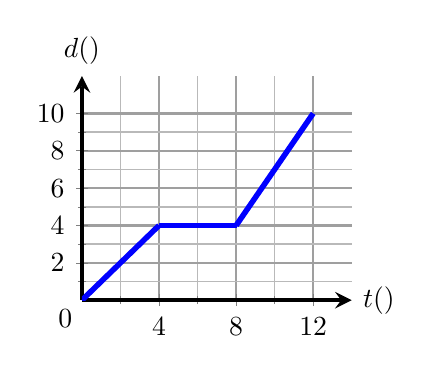
\begin{tikzpicture}  
			\begin{axis}[  ultra thick,scale=0.5,
				xmin=0,  
				xmax=14,  
				xtick={0,4,...,12},
				ytick={0,2,...,10},
				minor x tick num=1,
				minor y tick num=1,
				ymin=0,  
				ymax=12, 
				samples=300,
				axis lines=center, 
				grid style={step=1, line width =0.6pt, color=gray!55!white},
				grid=both, %giới hạn ô lưới
				major grid style={line width=0.8pt,gray!75!white},
				xlabel=$\xsi{t}{\left(\si{\second}\right)}$, 		ylabel=$\xsi{d}{\left(\si{\meter}\right)}$,
				every axis y label/.style={at=(current axis.above origin),anchor=south},  
				every axis x label/.style={at=(current axis.right of origin),anchor=west},  ]
				\addplot [line width=2pt, blue, smooth, domain=0:4] {x};  
				\addplot [line width=2pt, blue, smooth, domain=4:8] {4};
				\addplot [line width=2pt, blue, smooth, domain=8:12] {4+1.5*(x-8)};
				\coordinate (O) at (axis cs: 0,0);
			\end{axis}  
			\node[below left] at (O) {0};
	\end{tikzpicture}}
	\loigiai{}
\end{ex}
% ===================================================================
\begin{ex}
	Một vật chuyển động thẳng có đồ thị vận tốc theo thời gian như hình vẽ. Giai đoạn vật chuyển động thẳng nhanh dần đều là
	\begin{center}
		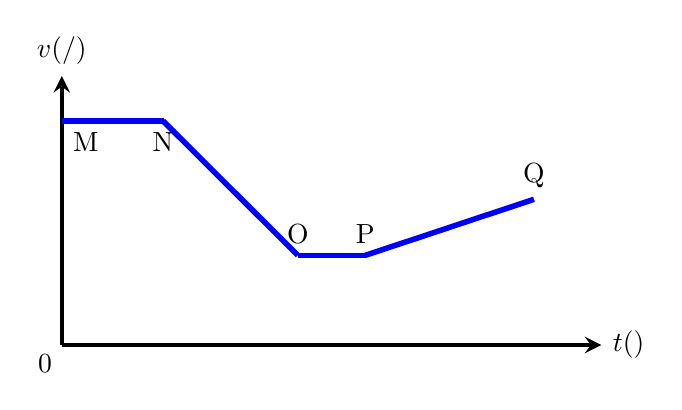
\begin{tikzpicture}  
			\begin{axis}[  ultra thick,yscale=0.6,
				xmin=0,  
				xmax=16,  
				ymin=0,  
				ymax=6, 
				samples=300,
				yticklabels=\empty,
				xticklabels=\empty,
				xtick=\empty,
				ytick=\empty,
				axis lines=center, 
				xlabel=$\xsi{t}{\left(\si{\second}\right)}$, 		ylabel=$\xsi{v}{\left(\si{\meter/\second}\right)}$,
				every axis y label/.style={at=(current axis.above origin),anchor=south},  
				every axis x label/.style={at=(current axis.right of origin),anchor=west},  ]
				\coordinate (M) at (axis cs: 0,5);
				\coordinate (N) at (axis cs: 3,5);
				\coordinate (OO) at (axis cs: 7,2);
				\coordinate (P) at (axis cs: 9,2);
				\coordinate (Q) at (axis cs: 14,3.25);
				\addplot [line width=2pt, blue, smooth, domain=0:3] {5}; 
				\addplot [line width=2pt, blue, smooth, domain=3:7] {5-0.75*(x-3)}; 
				\addplot [line width=2pt, blue, smooth, domain=7:9] {2}; 
				\addplot [line width=2pt, blue, smooth, domain=9:14] {2+0.25*(x-9)};
				\coordinate (O) at (axis cs: 0,0);
				\node[below right] at (M) {M};
				\node[below] at (N) {N};
				\node[above] at (OO) {O};
				\node[above] at (P) {P};
				\node[above] at (Q) {Q};
			\end{axis}  
			\node[below left] at (O) {0};
		\end{tikzpicture}
	\end{center}
	\choice
	{MN}
	{NO}
	{OP}
	{\True PQ}
	\loigiai{}
\end{ex}

% ===================================================================
\begin{ex}
	Bạn Bình đi học từ nhà đến trường theo lộ trình ABC như hình vẽ. Biết bạn Bình đi đoạn đường $\mathrm{AB}=\SI{400}{\meter}$ hết 6 phút, đoạn đường $\mathrm{BC}=\SI{300}{\meter}$ hết 4 phút. Vận tốc trung bình của bạn Bình khi đi từ nhà đến trường là
	\begin{center}
		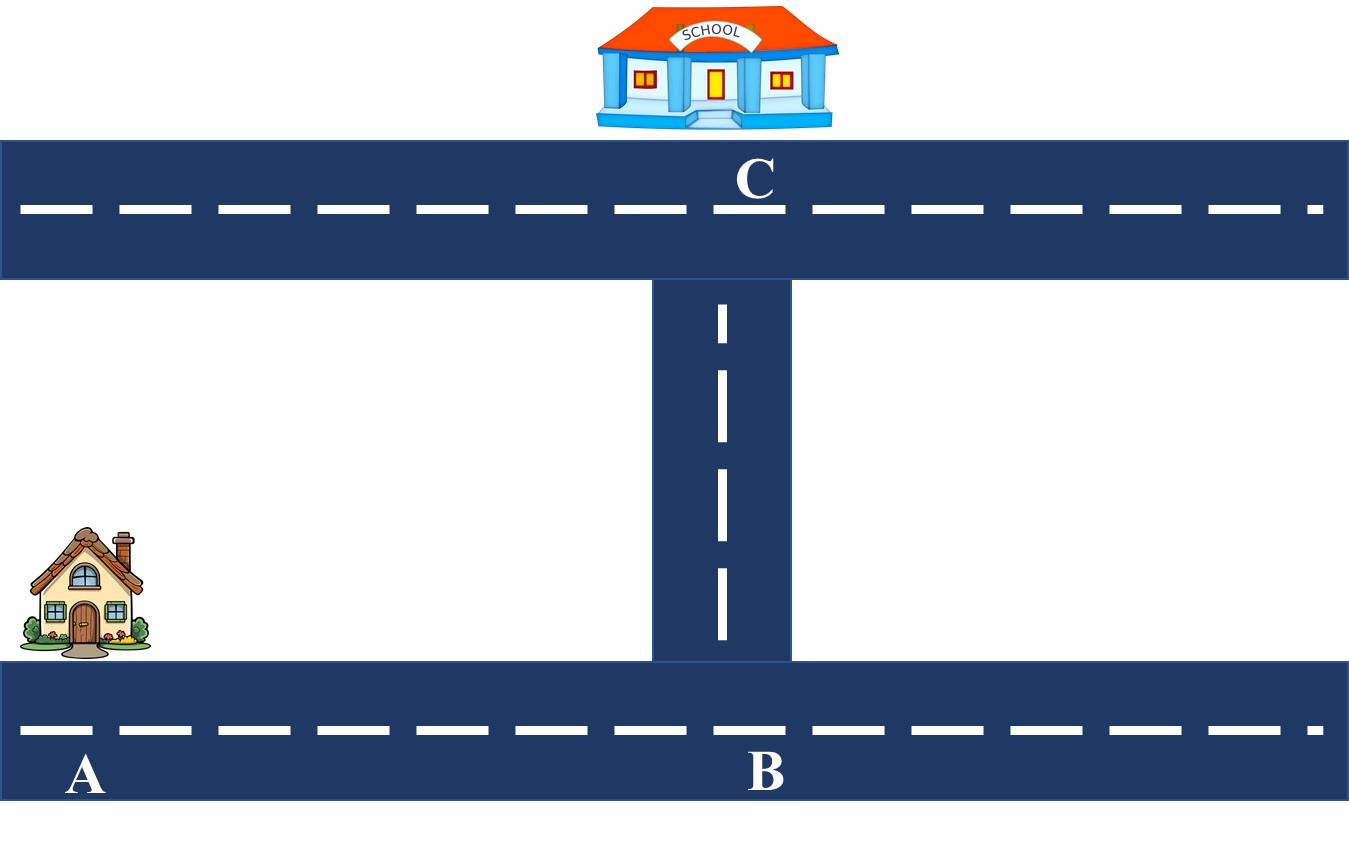
\includegraphics[width=0.4\linewidth]{../figs/D10-1-3}
	\end{center}
	\choice
	{\True $\SI{0.833}{\meter/\second}$}
	{$\SI{2.916}{\meter/\second}$}
	{$\SI{1.167}{\meter/\second}$}
	{$\SI{3.512}{\meter/\second}$}
	\loigiai{
		$$v=\dfrac{\mathrm{AC}}{t_{\mathrm{AB}}+t_{\mathrm{BC}}}\approx\SI{0.833}{\meter/\second}.$$
	}
\end{ex}
% ===================================================================
\begin{ex}
	Giờ Phối hợp Quốc tế (UTC) là tiêu chuẩn thời gian được sử dụng rộng rãi trên thế giới. So với 0 giờ Quốc Tế, Việt Nam ở múi giờ thứ 7 (UTC +7) và Nhật Bản ở múi giờ thứ 9 (UTC +9). Ngày 10/02/2024, máy bay VN300, thuộc hãng hàng không Vietnam Airlines, khởi hành từ Thành phố Hồ Chí Minh lúc 0 giờ 20 phút và đến Thành phố Tokyo lúc 7 giờ 45 phút, theo giờ địa phương. Thời gian di chuyển của máy bay này là
	\choice
	{\True 5 giờ 25 phút}
	{9 giờ 25 phút}
	{7 giờ 25 phút}
	{8 giờ 05 phút}
	\loigiai{
	}
\end{ex}

% ===================================================================
\begin{ex}
	Biểu thức nào sau đây đang mô tả vận tốc của vật chuyển động thẳng chậm dần đều?
	\choice
	{\True $v=-20+5t\ \left(\si{\meter/\second}; \si{\second}\right)$}
	{$v=10+5t\ \left(\si{\meter/\second}; \si{\second}\right)$}
	{$v=5t\ \left(\si{\meter/\second}; \si{\second}\right)$}
	{$v=-20-5t\ \left(\si{\meter/\second}; \si{\second}\right)$}
	\loigiai{}
\end{ex}
% ===================================================================
\begin{ex}
	Một vật chuyển động thẳng nhanh dần đều với tốc độ đầu là $\SI{6}{\meter/\second}$ và độ lớn gia tốc là $\SI{2}{\meter/\second^2}$. Chọn thời điểm ban đầu là lúc vật ở gốc tọa độ và chiều dương ngược chiều chuyển động thì phương trình chuyển động của vật có dạng
	\choice
	{$x=6t-t^2\ \left(\si{\meter}; \si{\second}\right)$}
	{$x=6t-2t^2\ \left(\si{\meter}; \si{\second}\right)$}
	{\True $x=-6t-t^2\ \left(\si{\meter}; \si{\second}\right)$}
	{$x=-6t-2t^2\ \left(\si{\meter}; \si{\second}\right)$}
	\loigiai{}
\end{ex}
% ===================================================================
\begin{ex}
	Một xe đi nửa đoạn đường đầu tiên với tốc độ trung bình
	$v_1=\SI{12}{\kilo\meter/\hour}$ và nửa đoạn đường	sau với tốc độ trung bình $v_2=\SI{20}{\kilo\meter/\hour}$. Tốc độ trung bình của xe trên cả đoạn đường là
	\choice
	{$\SI{30}{\kilo\meter/\hour}$}
	{\True $\SI{15}{\kilo\meter/\hour}$}
	{$\SI{16}{\kilo\meter/\hour}$}
	{$\SI{32}{\kilo\meter/\hour}$}
	\loigiai{
		$$v_{\text{tb}}=\dfrac{2s}{\dfrac{s}{v_1}+\dfrac{s}{v_2}}=\dfrac{2}{\dfrac{1}{v_1}+\dfrac{1}{v_2}}=\SI{15}{\kilo\meter/\hour}.$$
	}
\end{ex}
% ===================================================================
\begin{ex}
	Một ô tô đang chạy với vận tốc $\SI{72}{\kilo\meter/\hour}$ trên một đoạn đường thẳng thì người lái xe hãm phanh cho ô tô chạy chậm dần. Sau $\SI{40}{\second}$, ô tô dừng lại. Gia tốc của ô tô là
	\choice
	{$a=\SI{-0.2}{\meter/\second^2}$}
	{\True $a=\SI{-0.5}{\meter/\second^2}$}
	{$a=\SI{0.2}{\meter/\second^2}$}
	{$a=\SI{-1}{\meter/\second^2}$}
	\loigiai{
		$$a=\dfrac{v-v_0}{\Delta t}=\dfrac{0-20}{40}=\SI{-0.5}{\meter/\second^2}.$$
	}
\end{ex}

% ===================================================================
\begin{ex}
	Một xe máy đang chạy với tốc độ $\SI{36}{\kilo\meter/\hour}$ bỗng người lái xe thấy có một cái hố trước mặt, cách xe $\SI{20}{\meter}$. Người ấy phanh gấp và xe đến ngay trước miệng hố thì dừng lại. Gia tốc của xe máy có độ lớn là 
	\choice
	{$\SI{5.09}{\meter/\second^2}$}
	{$\SI{4.1}{\meter/\second^2}$}
	{\True $\SI{2.5}{\meter/\second^2}$}
	{$\SI{32.4}{\meter/\second^2}$}
	\loigiai{}
\end{ex}

% ===================================================================
\begin{ex}
	Một vật chuyển động trên đường thẳng có phương trình vận tốc - thời gian $v=-5+5t\ \left(\si{\meter/\second};\si{\second}\right)$. Tại thời điểm $t=\SI{10}{\second}$ thì quãng đường vật đã đi \textbf{gần nhất} với giá trị nào?
	\choice
	{$\SI{400}{\meter}$}
	{$\SI{300}{\meter}$}
	{$\SI{100}{\meter}$}
	{\True $\SI{200}{\meter}$}
	\loigiai{
		Thời điểm vật đổi chiều chuyển động: $v=0\Rightarrow t=\SI{1}{\second}$.\\
		Trong 1 giây đầu vật chuyển động chậm dần đều ngược chiều dương với vận tốc đầu $v_0=\SI{-5}{\meter/\second}$ và gia tốc $a=\SI{5}{\meter/\second^2}$: $d=v_0t+\dfrac{1}{2}at^2=\SI{-2.5}{\meter}\Rightarrow s=\SI{2.5}{\meter}$.\\
		Trong 9 giây còn lại vật chuyển động nhanh dần theo chiều dương với gia tốc $a=\SI{5}{\meter/\second^2}$:
		$s'=\dfrac{1}{2}at'^2=\SI{202.5}{\meter}$.\\
		Vậy tổng quãng đường dịch chuyển là $s+s'=\SI{205}{\meter}$.
	}
\end{ex}


% ===================================================================
\begin{ex}
	Các giọt nước mưa rơi từ một đám mây; khi xuống tới gần mặt đất	coi giọt mưa rơi thẳng đứng với tốc độ không đổi $\SI{30}{\meter/\second}$, lúc này giọt nước đập vào tấm kính ở cửa bên của một ô tô đang chuyển động thẳng đều theo phương ngang, giọt mưa để lại trên kính một vết nước hợp với phương thẳng đứng một góc $\SI{30}{\degree}$. Tốc độ của ô tô \textbf{gần nhất} với giá trị nào sau đây?
	\choice
	{\True $\SI{62.4}{\kilo\meter/\hour}$}
	{$\SI{108}{\kilo\meter/\hour}$}
	{$\SI{54.8}{\kilo\meter/\hour}$}
	{$\SI{72.5}{\kilo\meter/\hour}$}
	\loigiai{
		$$v_{\text{xe}}=v_{\text{mưa}}\cdot\tan\SI{30}{\degree}\approx\SI{62,4}{\kilo\meter/\hour}.$$
	}
\end{ex}


\Closesolutionfile{ans}
\section{Câu trắc nghiệm đúng/sai} 
\textit{Thí sinh trả lời từ câu 1 đến câu 2. Trong mỗi ý \textbf{a)}, \textbf{b)}, \textbf{c)}, \textbf{d)} ở mỗi câu, thí sinh chọn đúng hoặc sai}
\setcounter{ex}{0}
\Opensolutionfile{ans}[ans/D10-GKI-001-TF]

% ===================================================================
\begin{ex}
	Trong một tình huống bóng đá, thủ môn xuất phát từ vạch ngang nối hai cột của khung thành chạy thẳng lên phía trước để bắt bóng. Hình bên là đồ thị độ dịch chuyển - thời gian của thủ môn. Điểm A tương ứng với điểm xuất phát, đoạn AB có dạng parabol, BC là đoạn thẳng.
	\begin{center}
		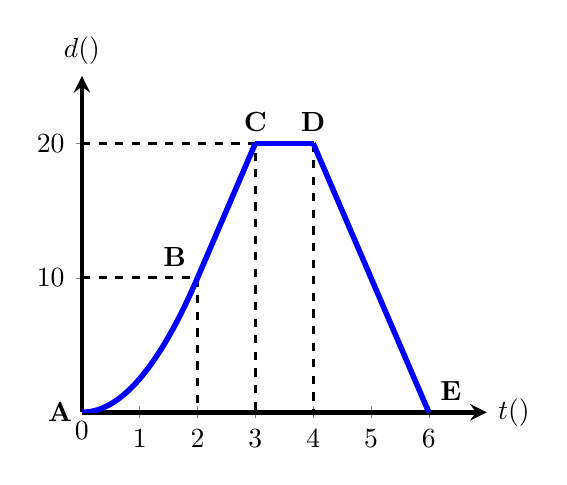
\begin{tikzpicture}  
			\begin{axis}[  ultra thick,scale=0.75,
				xmin=0,  
				xmax=7,  
				xtick={0,1,...,6},
				ytick={0,10,20},
				minor x tick num=0,
				minor y tick num=0,
				ymin=0,  
				ymax=25, 
				samples=300,
				axis lines=center, 
				xlabel=$\xsi{t}{\left(\si{\second}\right)}$, 		ylabel=$\xsi{d}{\left(\si{\meter}\right)}$,
				every axis y label/.style={at=(current axis.above origin),anchor=south},  
				every axis x label/.style={at=(current axis.right of origin),anchor=west},  ]
				\draw[dashed, line width=1pt] (axis cs: 0,10)--(axis cs: 2,10)--(axis cs: 2,0);
				\draw[dashed, line width=1pt] (axis cs: 0,20)--(axis cs: 3,20)--(axis cs: 3,0);
				\draw[dashed, line width=1pt] (axis cs: 4,20)--(axis cs: 4,0);
				\addplot [line width=2pt, blue, smooth, domain=0:2] {0.5*5*x^(2)}; 
				\addplot [line width=2pt, blue, smooth, domain=2:3] {10+10*(x-2)};  
				\addplot [line width=2pt, blue, smooth, domain=3:4] {20}; 
				\addplot [line width=2pt, blue, smooth, domain=4:6] {20-10*(x-4)};
				\coordinate (O) at (axis cs: 0,0);
				\coordinate (A) at (axis cs: 0,0);
				\coordinate (B) at (axis cs: 2,10);
				\coordinate (C) at (axis cs: 3,20);
				\coordinate (D) at (axis cs: 4,20);
				\coordinate (E) at (axis cs: 6,0);
				\node[above left] at (B) {\textbf{B}};
				\node[above] at (C) {\textbf{C}};
				\node[above] at (D) {\textbf{D}};
				\node[above right] at (E) {\textbf{E}};
			\end{axis}  
			\node[below] at (O) {0};
			\node[left] at (A) {\textbf{A}};
		\end{tikzpicture}
	\end{center}
	\choiceTF[t]
	{Trong khoảng thời gian từ $\SI{0}{\second}$ đến $\SI{6}{\second}$ thủ môn không đổi hướng chuyển động}
	{\True Thủ môn tăng tốc trong khoảng thời gian từ $\SI{0}{\second}$ đến $\SI{2}{\second}$}
	{\True Tốc độ chuyển động của thủ môn từ điểm B đến điểm C là $\SI{10}{\meter/\second}$}
	{\True Từ 4 giây đến 6 giây, vận tốc chuyển động của thủ môn có giá trị $\SI{-10}{\meter/\second}$}
	\loigiai{}
\end{ex}
% ===================================================================
\begin{ex}
	Khi xe chạy trên đường cao tốc, xe phải giữ khoảng cách an toàn với xe phía trước để có thể xử lý kịp thời khi xe phía trước gặp sự cố.
	\begin{center}
		
\includegraphics[width=0.4\linewidth]{../figs/D10-1-4}
	\end{center}	
	Khoảng cách an toàn này tùy thuộc vào tốc độ xe và đã được nêu trong một số quy định của chính phủ. Tuy nhiên, để dễ nhớ, khi lưu thông vào ban ngày và khi đường khô ráo người ta thường tính toán theo một trong các quy tắc sau:
	\begin{itemize}
		\item \textbf{\textit{Quy tắc 1:}} Quy tắc $\SI{3}{\second}$  tối thiểu. Khoảng cách an toàn tối thiểu bằng quãng đường xe đi được trong $\SI{3}{\second}$. Ví dụ xe chạy với tốc độ $\SI{72}{\kilo\meter/\hour}$  thì khoảng cách an toàn tối thiểu với xe phía trước là $\SI{60}{\meter}$.
		\item \textbf{\textit{Quy tắc 2:}} Quy tắc tương đương. Khoảng cách an toàn tối thiểu (theo đơn vị $\si{\meter}$) bằng tốc độ của xe (theo đơn vị $\si{\kilo\meter/\hour}$). Ví dụ tốc độ xe là $\SI{80}{\kilo\meter/\hour}$  thì khoảng cách an toàn tối thiểu với xe phía trước là $\SI{80}{\meter}$.
	\end{itemize}
	Một xe ô tô đang chạy trên đường cao tốc nằm ngang với tốc độ $\SI{108}{\kilo\meter/\hour}$  thì bất ngờ thấy một sự cố trên đường ở phía trước, sau đó $\SI{1}{\second}$ thì tài xế ô tô bắt đầu giảm hẳn ga và thắng gấp xe lại với gia tốc có độ lớn $\SI{8}{\meter/\second^2}$ cho đến khi xe ngừng lại.
	\choiceTF[t]
	{\True Theo quy tắc 1, khoảng cách an toàn tối thiểu với trường hợp xe ô tô trên là $\SI{90}{\meter}$}
	{Theo quy tắc 2, khoảng cách an toàn tối thiểu với trường hợp xe ô tô trên là $\SI{30}{\meter}$}
	{\True Tổng quãng đường ô tô đi được từ lúc phát hiện sự cố đến khi dừng lại $\SI{86.25}{\meter}$}
	{\True Nếu sự cố mà xe ô tô nhìn thấy là một xe container phía trước, đang chuyển động cùng chiều, thẳng đều, với tốc độ $\SI{36}{\kilo\meter/\hour}$ thì khoảng cách tối thiểu của hai xe kể từ lúc người lái ô tô thắng lại phải là $\SI{25}{\meter}$ để không xảy ra tai nạn. }
	\loigiai{
		\begin{itemchoice}
			\itemch Đúng.
			\itemch Sai. Theo quy tắc 2, khoảng cách an toàn tối thiểu là $\SI{108}{\meter}$.
			\itemch Đúng.\\
			Trong quá trình từ khi ô tô thấy sự cố đến khi thắng lại, ô tô chuyển động thẳng đều. Quãng đường ô tô đi được trong quá trình trên: $s_1=v_0t=30\cdot1=\SI{30}{\meter}$.\\
			Trong quá trình ô tô thắng lại, ô tô chuyển động chậm dần đều với vận tốc đầu $v_0$. Đến khi dừng lại  $v=0$.\\
			Quãng đường ô tô đi được trong quá trình này: $s_2=\dfrac{v^2-v^2_0}{2a}=\SI{56.25}{\meter}$.\\
			Tổng quãng đường ô tô đi được từ lúc phát hiện sự cố đến khi dừng lại: $s=s_1+s_2=\SI{86.25}{\meter}$.
			\itemch Đúng.\\
			Chọn trục tọa độ  gắn với xe con, chiều dương $Ox$ cùng chiều chuyển động của xe, gốc tọa độ O trùng với điểm B, gốc thời gian lúc ô tô bắt đầu hãm phanh.\\
			Phương trình chuyển động của ô tô: $x_1=-\mathrm{AB}+v_{01}t-\dfrac{1}{2}at^2$.\\
			Phương trình chuyển động của xe container:  $x_2=v_2t$.\\
			Nếu hai xe va chạm (gặp nhau): 
			$$x_1=x_1\Rightarrow \mathrm{AB}+\left(v_2-v_{01}\right)t+\dfrac{1}{2}at^2=0 \quad \left(*\right)$$
			Để ô tô chỉ gặp xe container một lần và dừng lại ngay trước khi va chạm, hoặc không gặp xe container (không xảy ra tai nạn) thì phương trình (*) phải có không quá một nghiệm thực, khi đó biệt số $\Delta $:
			$$\Delta \le 0\Leftrightarrow \left(v_2-v_{01}\right)^2-2a\cdot\mathrm{AB}\le 0$$
			$$\Rightarrow \mathrm{AB}\ge \dfrac{\left(v_2-v_{01}\right)^2}{2a}$$
			$$\Rightarrow \mathrm{AB}_{\text{min}}=\dfrac{\left(v_2-v_{01}\right)^2}{2a}=\SI{25}{\meter}.$$
		\end{itemchoice}
	}
\end{ex}
\Closesolutionfile{ans}

\section{Câu trắc nghiệm trả lời ngắn} \textit{Thí sinh trả lời từ câu 1 đến câu 6}
\setcounter{ex}{0}
\Opensolutionfile{ans}[ans/D10-GKI-001-TL]
% ===============================================================
\begin{ex}
	Một vận động viên chạy từ điểm xuất phát lên một quả đồi với tốc độ không đổi $\SI{3}{\meter/\second}$. Khi chạy được $\SI{90}{\meter}$ thì vận động viên này lập tức chạy ngược lại theo đường cũ về điểm xuất phát với tốc độ không đổi $\SI{6}{\meter/\second}$. Ở cả hành trình trên, tốc độ trung bình của vận động viên là bao nhiêu $\si{\meter/\second}$?
	\shortans{4 }
	\loigiai{
		$$v_{\text{tb}}=\dfrac{2s}{\dfrac{s}{v_1}+\dfrac{s}{v_2}}=\SI{4}{\meter/\second}.$$
	}
\end{ex}
% ===============================================================
\begin{ex}
	Một quả bóng tennis đang bay với tốc độ $\SI{25}{\meter/\second}$ theo hướng đông thì chạm vào tường chắn và bay trở lại với tốc độ $\SI{15}{\meter/\second}$ theo hướng tây. Thời gian va chạm giữa tường và bóng là $\SI{0.05}{\second}$. Tính gia tốc của quả bóng trong thời gian tiếp xúc với tường theo đơn vị $\si{\meter/\second^2}$. Chọn chiều dương là chiều chuyển động ban đầu của quả bóng.
	\shortans{-800 }
	\loigiai{
	}
\end{ex}
% ===============================================================
\begin{ex}
	Trong một thí nghiệm đo tốc độ chuyển động của vật nhỏ bằng đồng hồ cần rung, người ta đã thu được một băng giấy với các dấu mực như hình vẽ bên dưới. Thước đo được sử dụng trong hình vẽ là thước đo $\si{\centi\meter}$. Biết rằng khoảng thời gian giữa các lần chấm mực luôn bằng nhau và bằng $\SI{0.2}{\second}$. Trong khoảng thời gian giữa lần chấm mực đầu tiên (đánh số 1) cho đến lần chấm mực cuối cùng (đánh số 8) thì tốc độ trung bình của vật nhỏ đó bằng bao nhiêu $\si{\centi\meter/\second}$?	\textit{(Kết quả làm tròn đến 2 chữ số sau dấu phẩy thập phân)}.
	\begin{center}
		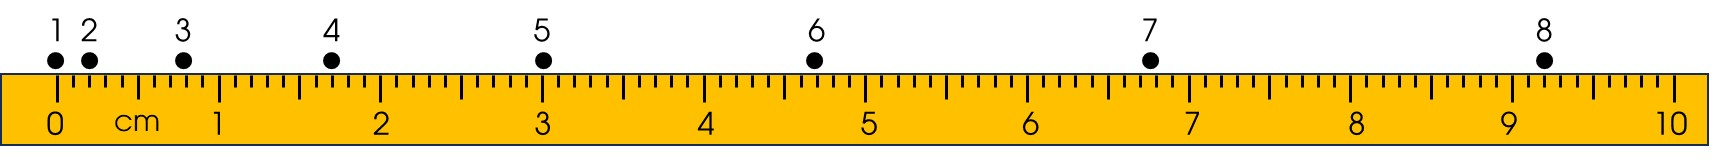
\includegraphics[width=0.9\linewidth]{../figs/D10-2-15}
	\end{center}
	\shortans{6,57}
	\loigiai{
		
	}
\end{ex}

% ===============================================================
\begin{ex}
	Một vật chuyển động thẳng có đồ thị vận tốc - thời gian như hình bên dưới. Tính tổng quãng đường vật đi được trong khoảng thời gian $\SI{12}{\second}$ theo đơn vị mét.
	\begin{center}
		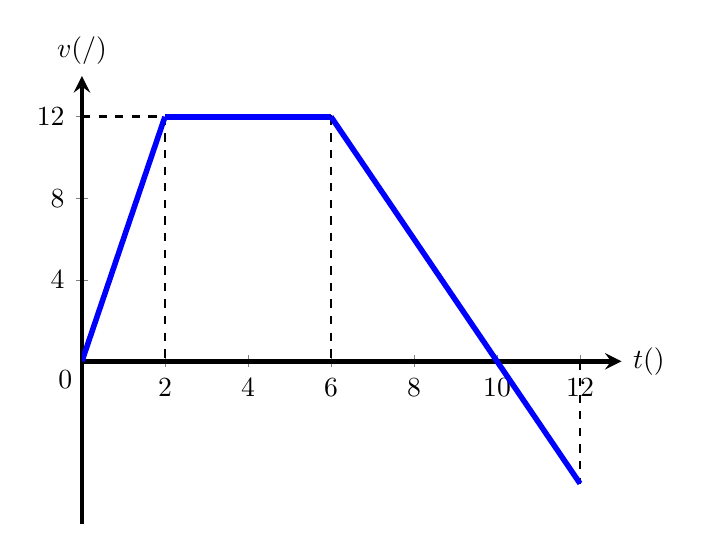
\begin{tikzpicture}  
			\begin{axis}[  ultra thick,
				xmin=0,  
				xmax=13,  
				xtick={0,2,...,12},
				ytick={0,4,...,12},
				ymin=-8,  
				ymax=14, 
				samples=300,
				axis lines=center, 
				xlabel=$\xsi{t}{\left(\si{\second}\right)}$, 		ylabel=$\xsi{v}{\left(\si{\meter/\second}\right)}$,
				every axis y label/.style={at=(current axis.above origin),anchor=south},  
				every axis x label/.style={at=(current axis.right of origin),anchor=west},  ]
				\draw[dashed, line width=1pt] (axis cs: 0,12)--(axis cs: 2,12)--(axis cs: 2,0);
				\draw[dashed, line width=1pt] (axis cs: 0,12)--(axis cs: 6,12)--(axis cs: 6,0);
				\draw[dashed, line width=1pt] (axis cs: 12,0)--(axis cs: 12,-6);
				\addplot [line width=2pt, blue, smooth, domain=0:2] {6*x}; 
				\addplot [line width=2pt, blue, smooth, domain=2:6] {12};  
				\addplot [line width=2pt, blue, smooth, domain=6:12] {12-3*(x-6)}; 
				\coordinate (O) at (axis cs: 0,0);
			\end{axis}  
			\node[below left] at (O) {0};
		\end{tikzpicture}
	\end{center}	
	\shortans{$90$ }
	\loigiai{
		$$s=\dfrac{1}{2}\cdot\left(4+10\right)\cdot12+\dfrac{1}{2}\cdot2\cdot6=\SI{90}{\meter}.$$
	}
\end{ex}
% ===================================================================
\begin{ex}
	Một người đi xe đạp với tốc độ $v_1=\SI{5}{\meter/\second}$ bên cạnh đường ray tàu hỏa thì thấy một chiếc tàu hỏa chạy qua cùng chiều. Tốc độ của tàu hỏa là $v_2=\SI{15}{\meter/\second}$ đối với mặt đất. Sau thời gian $\SI{15}{\second}$ thì người đó thấy tàu hỏa vượt qua mặt mình. Chiều dài của tàu hỏa là bao nhiêu mét?
	\begin{center}
		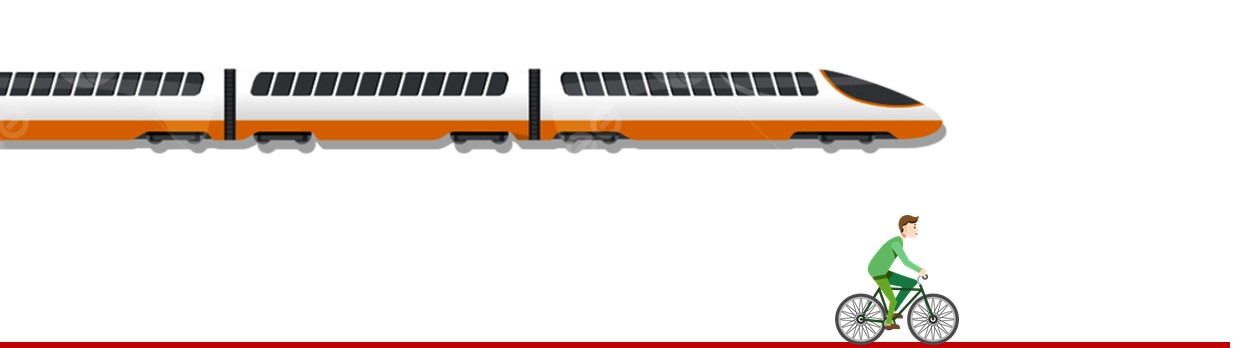
\includegraphics[width=0.5\linewidth]{../figs/D10-1-2}
	\end{center}
	\shortans{150}
	\loigiai{
		Vận tốc tương đối của tàu hỏa so với người:
		$$v_{21}=v_2-v_1=\SI{10}{\meter/\second}$$
		Chiều dài của tàu hỏa:
		$$L=v_{21}t=\SI{150}{\meter}.$$
	}
\end{ex}
% ===================================================================
\begin{ex}
	\immini{
		Trong khi làm thí nghiệm với đồng hồ đo thời gian hiện số, một học sinh chọn kiểu làm việc (MODE) của đồng hồ ở vị trí A và nối cổng quang điện với ổ A của đồng hồ. Học sinh này thả rơi một thước nhôm dài $\SI{20}{\centi\meter}$ theo phương thẳng đứng sao cho thước rơi qua cổng quang điện (thước luôn thẳng đứng khi rơi) thì thấy số chỉ của đồng hồ bằng $\SI{0.077}{\second}$. 
	}
	{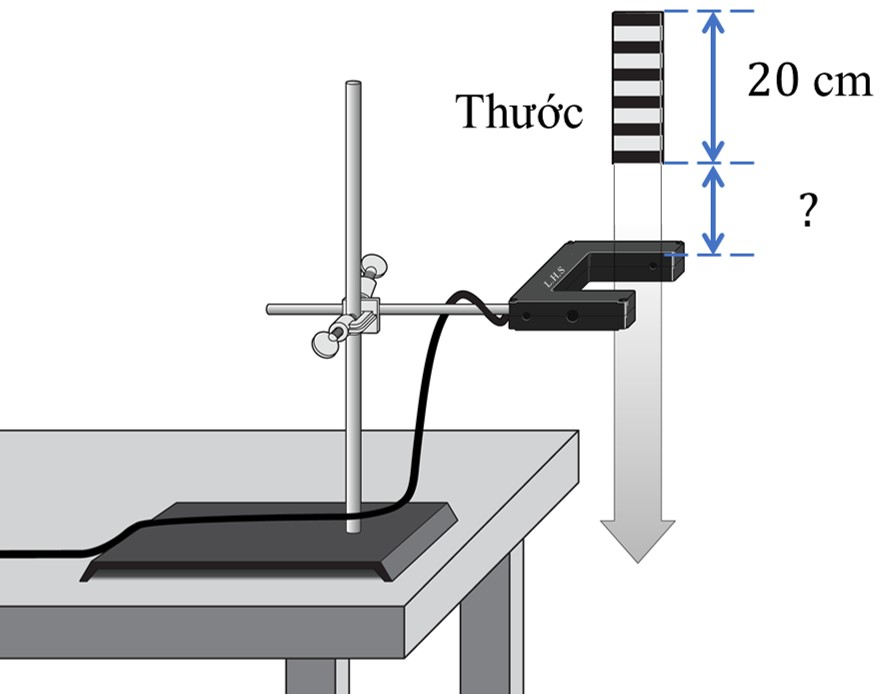
\includegraphics[width=0.6\linewidth]{../figs/D10-1-1}}
	Bỏ qua sức cản của không khí và thước chuyển động nhanh dần đều với gia tốc có độ lớn $\SI{9.8}{\meter/\second^2}$. Khi thả, đầu dưới của thước cách cổng quang điện một khoảng bằng bao nhiêu? \textit{(Kết quả tính theo đơn vị centimet và làm tròn đến phần nguyên.)}
	\shortans{25}
	\loigiai{
		Gọi $v$ là vận tốc của thước khi đầu thước bắt đầu chắn qua cổng quang thì:
		$$\ell=vt+\dfrac{1}{2}at^2\Leftrightarrow 0,2=v\cdot0,072+\dfrac{1}{2}\cdot9,8\cdot0,072^2\Rightarrow v\approx\SI{2.22}{\meter/\second}.$$
		Khoảng cách từ đầu thước đến cổng quang lúc thả:
		$$h=\dfrac{v^2}{2a}\approx\SI{0.25}{\meter}=\SI{25}{\centi\meter}.$$
	}
\end{ex}

\Closesolutionfile{ans}
\begin{center}
	\textbf{-- HẾT --}
\end{center}
\newpage
\setcounter{section}{0}
\begin{center}
	\textbf{\large BẢNG ĐÁP ÁN}
\end{center}
\section{}
\inputansbox{10}{ans/D10-GKI-001-TN}
\section{}
\inputansbox[2]{2}{ans/D10-GKI-001-TF}
\section{}
\inputansbox[3]{6}{ans/D10-GKI-001-TL}